\chapter*{\label{ref-009}De liefde}


 Voor Joop heb ik een ander vriendje gehad me wie ik wel serieus was. Hij woonde in Warmenhuizen maar dat heb ik na een poosje uitgemaakt. Ik wilde nog van alles, reizen en werken en hij wilde al trouwen en settelen en daar was ik nog niet aan toe. En na hem kwam Joop. 

 \begin{figure}[h]
    \begin{centering}
    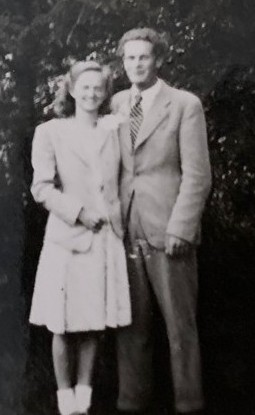
\includegraphics[width=0.5\textwidth]{image36}
    \caption{First love.}
    \end{centering}
\end{figure}

Hoe Joop en ik elkaar ontmoet hebben? Dat is wel een leuk verhaal. Hij was thuis met studieverlof voor zijn tweede rang. Hij had eerder een keer een reis met mijn broer gemaakt en toen kwamen ze tot de ontdekking dat ze beiden een zus hadden. Hij had toen eens een foto van mij gezien en vond me er kennelijk wel leuk uitzien.

En toen heeft hij mee een kaart geschreven, die hij naar Huis Ter Wege stuurde waar ik werkte. Hij schreef dat hij graag een afspraak wilde maken, en dat vond ik wel leuk! Ik vond het niet heel gek of eng want ik wist dat Kees hem wel kende. Dus het was niet zomaar echt helemaal een onbekende voor me. En ik geloof dat ik hem ook ooit eens gezien heb, op een feest van Kees. 


\begin{figure}[h]
    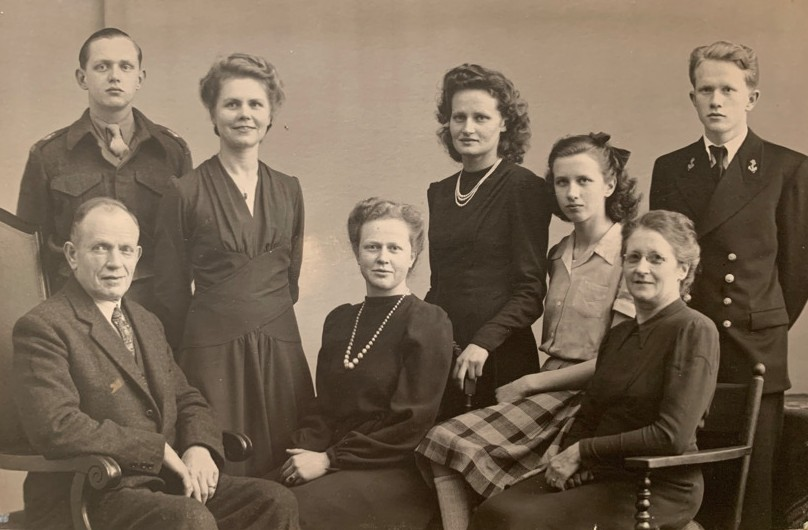
\includegraphics[width=\textwidth]{image37}
    \caption{Joop met zijn ouders en broer en zussen.}
\end{figure}

Hij was op zoek, dat was wel duidelijk. Dus we hebben een afspraak gemaakt in Utrecht. Toen ik hem zag vond ik hem er wel gelijk leuk uitzien, we zijn ergens gaan zitten koffiedrinken en hebben uren gepraat. 

We hebben eigenlijk maar heel weinig gewandeld kan ik me herinneren omdat we zoveel aan het praten waren. Hij bracht me met de taxi terug naar huis, terwijl ik gewoon met de trein naar Utrecht was gekomen. 

Het was al avond toen ik terugging dus toen vond hij het beter als ik met de taxi ging. Dat vond ik wel netjes van hem. Hij is in de taxi blijven zitten en niet eens mee naar binnen komen omdat het al laat was, maar daarna hebben we veel meer afspraakjes gehad. 

Ik viel op hem omdat hij leuk kon praten, hij kon leuk dingen vertellen en hij was hartstikke lief voor me. Het is heel anders als je een vriend hebt die vaart natuurlijk, dan was het echt feest als hij weer even verlof had.

Dan gingen we leuke dingen doen. Dan zei ik wel dat we niet altijd op stap hoefden te gaan, maar hij zei dat dat juist wel moest omdat daar niks meer van zou komen als we kinderen hadden. We moesten er nog maar van genieten, zei hij.

We deden niets bijzonders, want we vonden het eigenlijk gewoon al geweldig om bij elkaar te kunnen zijn. Maar maakten gewoon uitstapjes. 

Ik mocht hem alleen niet meenemen naar de bioscoop, want daar hield hij niet van. Maar we gingen wel naar de schouwburg, in Amsterdam waar we ook een keertje in een hotel hebben geslapen. Dat was echt heel leuk.

We kenden elkaar eigenlijk nog helemaal niet zo lang toen en toen moest hij een jaar naar Zuid-Afrika.

Dat vond ik erg spannend en ook wel moeilijk, maar door een geluk bij een ongeluk kwam hij al veel eerder naar huis omdat hij malaria kreeg. Daar werd hij erg ziek van en toen wilde ze vanuit de maatschappij dat hij naar Nederland kwam tot hij weer beter was.

Als hij weg was schreven we elkaar. We hebben wat afgeschreven toen hij voer, dat was het enige communicatiemiddel dat er was. Tegenwoordig kun je een stuk gemakkelijker communiceren, maar als hij op reis was, was hij ook echt w\'{e}g. En dus konden we alleen in contact blijven door elkaar brieven te schrijven. 

Hij heeft weleens gebeld, maar dat wilde ik niet meer want dan hoorde ik zijn stem wel maar was hij er niet en dan miste ik hem een stuk meer dan wanneer we gewoon alleen maar schreven. Dus toen hebben we afgesproken dat we niet meer gingen bellen. 

Wel heeft hij ooit eens iets bijzonders gedaan, en dat is flessenpost sturen. Hij had de fles ergens in Itali\"{e} in de buurt van vissersschepen in het water gegooid, en hij had gezien dat die vissers de fles uit het water hadden gehaald. 

Hij had er wat geld in gedaan zodat de vissers de brief ook zouden posten en zo is hij bij mij aangekomen. Dat was wel heel bijzonder, dat was een brief op een onverwachts moment. Dat was dus een hele leuke verrassing kan ik me nog herinneren.

Soms duurde het wel een week voor ik een brief ontving als hij vertrok vanuit Rotterdam. En ik stuurde dan een brief terug, want ik kreeg een lijst met alle havens die hij aandeed onderweg. 

We hebben heel wat afgeschreven, maar ik heb ze niet bewaard. Ik vind dat het iets tussen ons twee\"{e}n is. Achteraf had ik ze misschien wel moeten bewaren, maar ik heb ze allemaal verbrand omdat het me heel naar lijkt dat anderen ze zouden kunnen lezen. 

Ik liep eens met Jacqueline langs een tweedehands winkel en in de etalage lagen oude brieven en dat deed me beseffen dat ik niet zou willen dat mijn brieven zo zouden belanden als ik er niet meer ben, vandaar.


En toen zijn we getrouwd. Maar van het aanzoek kan ik me eigenlijk nog maar weinig herinneren. We waren hartstikke verliefd maar hij ging niet op zijn knie\"{e}n met een ring, ik weet niet eens meer hoe dat ging. Het was wel leuk hoor! 

\begin{figure}[h]
    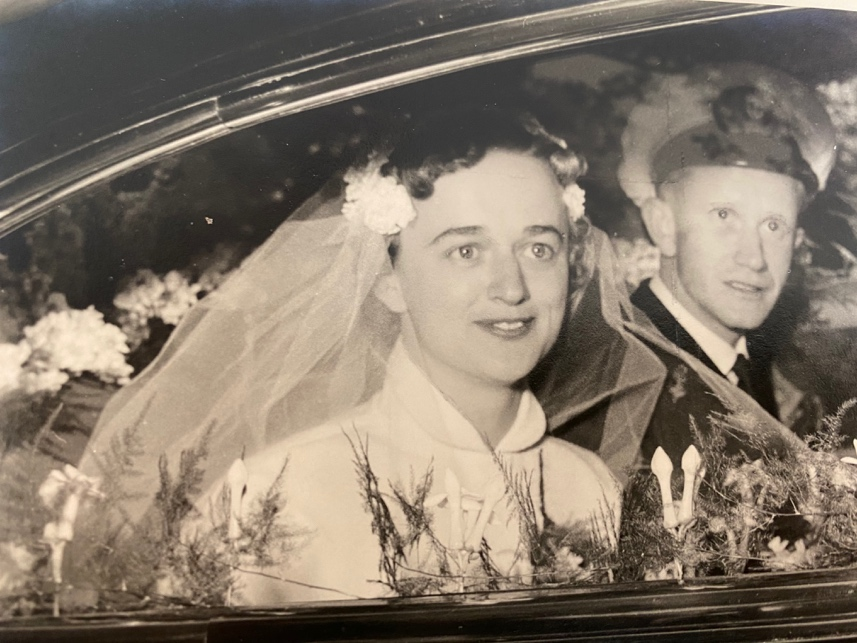
\includegraphics[width=\textwidth]{image41}
    \caption{Net getrouwd.}
\end{figure}

Het liep gewoon natuurlijk zo omdat we elkaar leuk vonden. Ik had het ook niet gewild dat hij op zijn knie\"{e}n ging, dat had ik verschrikkelijk gevonden. Ik vind dat belachelijk, dat een man op zijn knie\"{e}n moet gaan, je doet het toch samen? Ik had hem z\'{o} in zijn kraag gepakt en gezegd dat hij gauw weer moest gaan staan!

\begin{figure}[h]
    \begin{centering}
    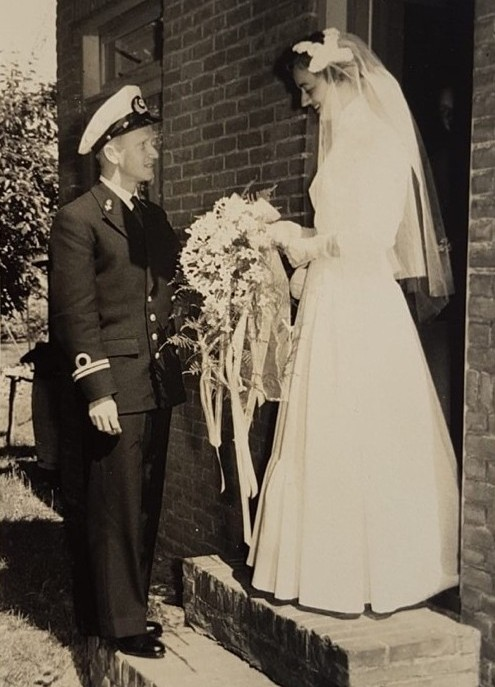
\includegraphics[width=.6\textwidth]{image38}
    \caption{Joop komt mij ophalen op onze huwelijksdag.}
    \end{centering}
\end{figure}

\begin{figure}[h]
    \begin{centering}
    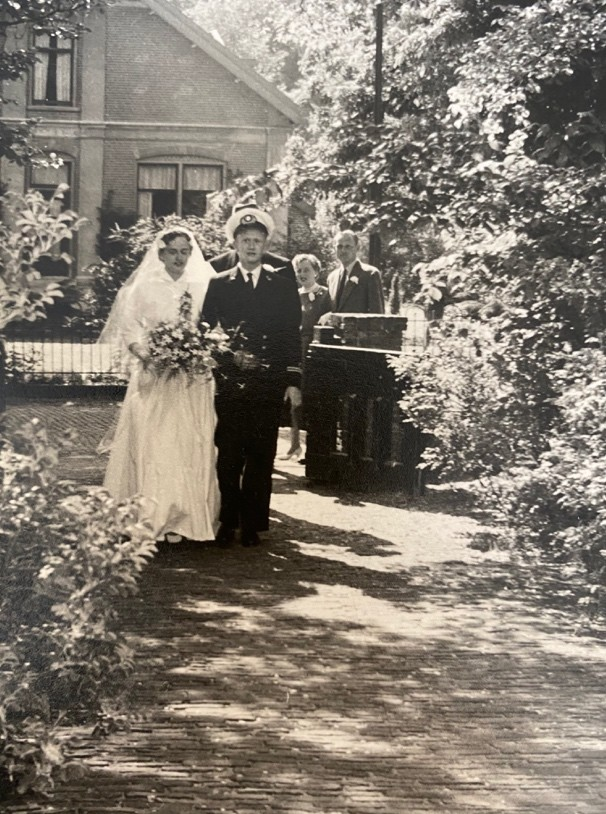
\includegraphics[width=\textwidth]{image39}
    \caption{De huwelijksceremonie!}
    \end{centering}
\end{figure}

% \begin{figure}[h]
%     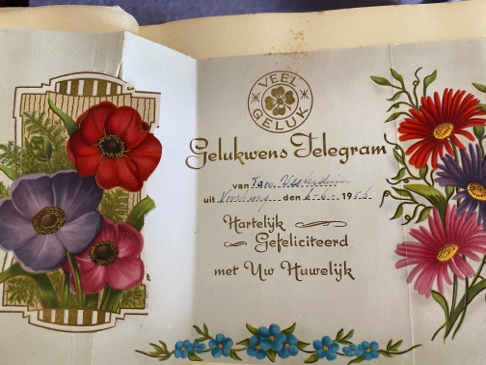
\includegraphics[width=\textwidth]{image40}
%     \caption{Gelukswens-Telegram.}
% \end{figure}

We zijn getrouwd in 1956, in Schoorl. De trouwjurk heb ik met mijn moeder in de Bijenkorf in Amsterdam gekocht, Het duurde niet heel lang tot ik hem had gevonden, ik vond hem gelijk die middag wel.

Over de trouwdag zelf weet ik niet heel veel meer. Ik denk dat ik wel zenuwachtig was maar dat weet ik echt niet meer. De hele familie van mij en Joop kwam, en het was wel een hele mooie dag. 

Hij droeg zijn uniform, en zag er heel mooi uit. Het scheelde ook in kosten, want zo hoefde hij niet nog een duur pak te kopen. Na het huwelijk hadden we een diner in een restaurant en dat was heel leuk en gezellig in kleine setting.

\begin{figure}[h]
    \begin{centering}
    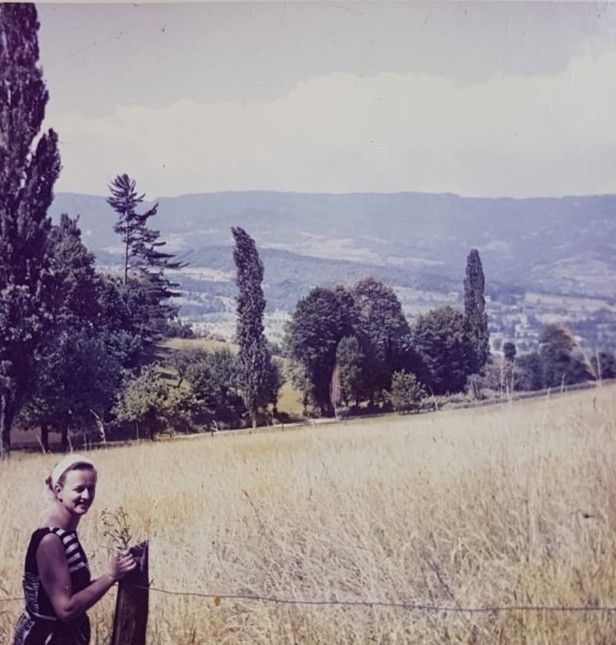
\includegraphics[width=\textwidth]{image42}
    \caption{Op huwelijksreis in Chamonix.}
    \end{centering}
\end{figure}
 
Na ons trouwen zijn we op huwelijksreis geweest in Frankrijk.

We wilden niet direct aan kinderen beginnen, maar ik was 29 dus dat vond ik wel een mooie leeftijd om moeder te worden. Maar toen de kinderen er net waren moest Joop alweer varen.

Dit was natuurlijk niet fijn, maar ik wist dat het zo zou lopen en was het al gewend dat hij langere periodes wegging. Dan stonden we te wuiven en ging hij weer.

Ik was altijd wel verdrietig en zou hem erg missen, maar ik moest niet huilen als hij wegging. Dat wilde ik hem niet aandoen. 

En toen veel later zijn we naar Valthe verhuisd. Toen we in Valthe zijn gaan wonen voer hij ook nog, maar toen werd hij ziek. Hij kreeg last van zijn keel, ik herinner me dat niet allemaal meer hoor. We wisten al wel snel dat het niet goed was.

Als ik terugkijk op ons huwelijk was het wel fijn, maar hij heeft natuurlijk wel veel gevaren en dat is niet leuk. Maar als hij thuis was was het wel heel fijn. Dan was het echt feest en genoot ik heel erg van het samenzijn.

En de mooiste herinnering die ik heb aan hem en ons? Dat is toch dat ik aan de kade stond en dat het schip weer aankwam waarop hij zat, nadat hij een jaar gevaren had. Dat gevoel was zo fijn, dat kan ik me nog precies voor de geest halen.
